\subsection{سوال 1}

\begin{enumerate}
	\item {
	      نموداری رسم کنید که محور افقی آن تعداد داده در batch-mini و محور عمودی آن تعداد گام لازم
	      برای همگرایی توسط الگوریتم SGⅮ جهت رسیدن به مقدار از پیش تعیین شده ای از خطای آموزش
	      باشد. بخش آغازین نمودار (بسته های کوچک داده) و بخش پایانی نمودار (بسته های بزرگ داده) را
	      با ذکر دلیل توجیه نمایید.

	      \begin{qsolve}[]
		      \begin{minipage}{0.5\textwidth}
			      به طور کلی، افزایش اندازه بسته mini-batch می‌تواند به سریع تر به همگرایی منجر شود،
			      اما همچنین به افزایش مصرف حافظه محاسباتی نیاز دارد.
			      این تجزیه و تحلیل به معنای این است که انتخاب اندازه مناسب برای mini-batch در SGD نیازمند تعادل بین سرعت همگرایی و میزان حافظه مورد نیاز است.

			      \[
				      \theta_{i+1} = \theta_i - \eta \nabla J(\theta_i, x^{(i)}, y^{(i)})
			      \]

			      افزایش سایز mini-batch منجر به سخت تر شدن محاسبه $\nabla J(\theta_i, x^{(i)}, y^{(i)})$ شده و همچنین مقدار $\theta_i$
			      بیشتری باید آپدیت شوند، در نتیجه حجم محاسبه بیشتر شده، ولی گرادیان محاسبه شده پرمعنا تر است.

			      بررسی بیشتر در: \cite{tsukada2023relationship}
		      \end{minipage}
		      \hspace*{2em}
		      \begin{minipage}{0.45\textwidth}
			      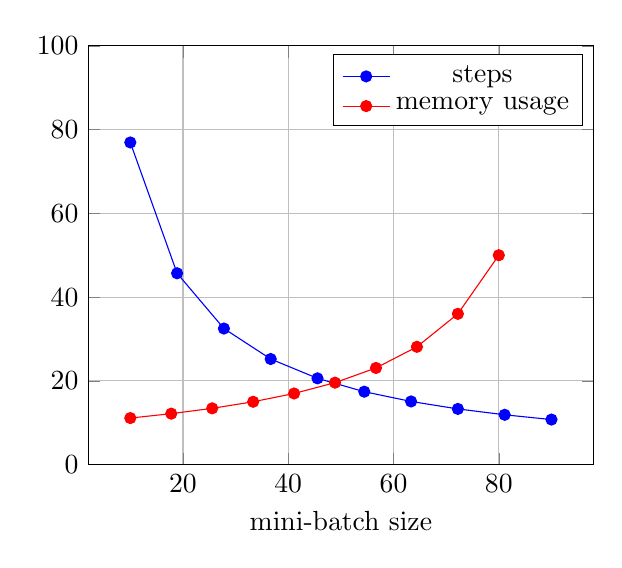
\begin{tikzpicture}
				      \begin{axis}[
						      xlabel={mini-batch size},
						      ymin=0, ymax=100, % You can adjust the y-axis limits as needed
						      grid=both,
						      width=8cm,
					      ]

					      \addplot[mark=*,blue,domain=10:90,samples=10] {1000/(x+3)};
					      \addplot[mark=*,red,domain=10:80,samples=10] {1000/(100-x)};

					      \legend{steps, memory usage}
				      \end{axis}

			      \end{tikzpicture}
		      \end{minipage}
	      \end{qsolve}

	      }
	\item {
	      آیا می توان گفت که در لایه Normalization Batch و در هنگام آموزش، مقداری نویز به توابع فعالیت
	      لایه های مخفی تزریق می شود؟ چرا؟

	      \begin{qsolve}[]
			به این موضوع در مقاله ی \cite{luo2019understanding} به طور عمیق پرداخته شده است.
			
			به طور خلاصه ولی، انتخاب batch در روش \lr{Batch Normalization} یک عمل تصادفی است، 
			صورت مسئله روش BN به صورت زیر است:

			\[
				y=g(\hat{h}),\quad \hat{h}=\gamma \bar{h} + \beta,\quad \bar{h} = \frac{h-\mu_{\mathcal{B}}}{\sigma_{\mathcal{B}}}	
			\]

			حال چون انتخاب $\mathcal{B}$ خود یک کار تصادفی است، خود $\mu_{\mathcal{B}}$ و $\sigma_{\mathcal{B}}$ متغیرهای تصادفی خواهند بود.

			اگر سایز batch را بزرگ بگیریم، میتوان طبق قضیه حد مرکزی نشان داد که(اثبات دقیق تر در \cite{teye2018bayesian}): 

			\[
				\mu_{\mathcal{B}}\sim\mathcal{N}(\mu_{\mathcal{P}}, \frac{\sigma_{\mathcal{P}}}{M}),
				\quad 
				\sigma_{\mathcal{B}}\sim\mathcal{N}(\sigma_{\mathcal{P}}, \frac{{\rho+2}}{4M}),
				\quad 
				\rho:\text{kurtosis},
				\quad
				\mathcal{P}:\text{population}
			\]

			\splitqsolve
			
			حال به گونه ای میتوان دید که $y=g(\hat{h})$ نیز یک متغیر تصادفی خواهد شد، باز اگر M بزرگ باشد، میتوان به طور تقریبی از حد مرکزی 
			دید که:

			\[
				y\sim\mathcal{N}(y_\mathcal{P}, \sigma)=y_{\mathcal{P}}+\mathcal{N}(0, \sigma),\quad
				y_{\mathcal{P}}=g\left(\gamma\frac{h-\mu_{\mathcal{P}}}{\sigma_{\mathcal{P}}}+\beta\right)
			\]

			پس میتوان چنین تعبیری کرد که در واقع این عملیات BN مانند نویزی کردن توابع فعالیت است، جزئیات محاسبه $\sigma$ 
			در اینجا آورده نشده است.

			\[
				g(\hat{h})=g(\hat{h_{\mathcal{P}}})+\delta,\quad \delta\sim\mathcal{N}(0,\sigma)
			\]
	      \end{qsolve}
	      }

	    %   \clearpage
	\item {
	      شبکه ی عصبی Connected Fully ای را درنظر بگیرید که تمام توابع فعالیت آن سیگموید باشد و وزن
	      های اولیه آن مقادیر مثبت بزرگ باشد. آیا این شبکه مناسبی برای طبقه بندی می باشد؟ چرا؟

	      \begin{qsolve}[]

		      یک شبکه عصبی Connected Fully با تمام توابع فعالیت سیگموید و وزن‌های اولیه مثبت بزرگ، عموماً مناسب برای تمام مسائل طبقه‌بندی نیست. این مسئله به عوامل زیر بستگی دارد:

		      \begin{itemize}
			      \item
			            پیچیدگی توابع هدف: برای مسائل با توابع هدف پیچیده و غیرخطی، توانایی یک شبکه با توابع فعالیت سیگموید محدودتر است و نیاز به توانایی‌های شبکه‌های عمیق‌تر مانند شبکه‌های عصبی با لایه‌های ReLU دارد.

			      \item
			            وزن‌های اولیه بزرگ ممکن است باعث مشکلاتی مانند سریع برخورد به واحدهای اشباع (saturation) در توابع سیگموید شوند و منجر به کندی در آموزش یا برخورد به مشکل گرادیان نزولی شود.

			      \item نوع داده‌ها نیز تأثیر دارد. برای مسائل مانند تشخیص تصاویر، شبکه‌های کانولوشنال با ویژگی‌های مربوط به تصاویر بهتر عمل می‌کنند.

			      \item اگر تعداد ورودی‌ها بسیار بزرگ باشد، این نوع شبکه ممکن است به مشکلات مصرف
		      \end{itemize}

		      به طور خلاصه، این شبکه ممکن است برای مسائل ساده و کوچک مناسب باشد، اما برای بسیاری از مسائل پیچیده و مهم، نیاز به شبکه‌های عمیق‌تر و تنوع‌تر با توابع فعالیت متنوع‌تر داریم. همچنین وزن
		      های اولیه بزرگ در توابع فعالیت سیگموید منجر به saturation و کم شدن گرادیان ها و \lr{vanishing gradient} شده پس این نوع مقدار دهی نیز کار ما را سخت تر میکند.
	      \end{qsolve}
	      }
	\item {
	      شبکه ی عصبی Connected Fully ای با 5 لایه مخفی، که در هر کدام از لایه ها، 10 نورون وجود
	      دارد را در نظر بگیرید. ورودی این شبکه ۲۰ بعدی و خروجی آن اسکالر می باشد. تعداد کل پارامتر
	      های قابل آموزش را در این شبکه محاسبه کنید.

	      \begin{qsolve}[]
		      \begin{latin}
				\small
			      \begin{align*}
				      \text{Total Trainable Parameters} & = (I_0 \times H_1 + H_1) + (\overbrace{H_1 \times H_2}^{\text{Weights}} + \overbrace{H_2}^{\text{biases}}) + (H_2 \times H_3 + H_3) \\
				                                        & + (H_3 \times H_4 + H_4) + (H_4 \times H_5 + H_4) + (H_5 \times O + O)
			      \end{align*}
		      \end{latin}
		      \vspace*{-0.8em}
			  پس برای این مسئله داریم که:
		      \vspace*{-1.2em}
		      \begin{latin}
				\small
			      \begin{align*}
				      \text{Total Trainable Parameters} & = (20 \times 10 + 10) + (10 \times 10 + 10) + (10 \times 10 + 10) \\
				                                        & + (10 \times 10 + 10) + (10 \times 10 + 10) + (10 \times 1 + 1) = 661
			      \end{align*}
		      \end{latin}

	      \end{qsolve}
	      }
	\item {
	      یک مسئله طبقه بندی باینری می تواند با دو روش زیر حل شود:

	      \textbf{روش اول: } \lr{Logistic regression} ساده (یک نورون)

	      \hspace*{2em}
	      خروجی: $\hat{y}=\sigma(W_lx+b_l)$

	      \hspace*{2em}
	      اکر $\hat{y}\leq 0.5$ کلاس صفر در غیر این صورت کلاس یک طبقه بندی می شود.

	      \textbf{روش ذوم: } \lr{Softmax regression} ساده (دو نورون)

	      \hspace*{2em}
	      خروجی: $\hat{y}=Softmax(W_sx+b_s)=[\hat{y}_1,\hat{y}_2]^T$

	      \hspace*{2em}
	      اکر $\hat{y}_1\geq\hat{y}_2$ کلاس صفر در غیر این صورت کلاس یک طبقه بندی می شود.

	      روش دوم دو برابر روش اول پارامتر دارد. آیا می توان گفت که روش دوم مدل های پیچیده تری
	      نسبت به روش اول یاد می گیرد؟

	      اگر بله، پارامترهای  $(W_s, b_s)$ تابعی که روش دوم می تواند آن را مدل کند مثال بزنید در غیر این صورت
	      نشان دهید که $(W_s, b_s)$ همیشه میتواند برحسب $(W_l, b_l)$ نوشته شود.

	      \begin{qsolve}[]
		      مدل‌های \lr{Logistic Regression} و \lr{Softmax Regression} به عنوان دو روش مختلف در مسائل طبقه‌بندی باینری و چند دسته‌ای به کار می‌روند. اما اگر به دقت به معادلات داخلی این دو مدل نگاه کنیم، متوجه می‌شویم که این دو مدل در واقع دقیقاً یکی هستند و تنها با تغییراتی در وزن‌ها و بایاس‌ها به یکدیگر تبدیل می‌شوند.

		      در Softmax Regression، ما داریم:

		      \[
			      \hat{y}_1 = \frac{e^{(W_{s1}x + b_{s1})}}{e^{(W_{s1}x + b_{s1})} + e^{(W_{s2}x + b_{s2})}}=\frac{1}{1 + e^{[(W_{s2}-W_{s1})x + b_{s2}-b_{s1}]}}
		      \]

		      \[
			      \hat{y}_2 = \frac{e^{(W_{s2}x + b_{s2})}}{e^{(W_{s1}x + b_{s1})} + e^{(W_{s2}x + b_{s2})}}=1-\hat{y}_1\Rightarrow \hat{y}_1\geq\hat{y}_2\sim\hat{y}_1\geq0.5
		      \]

		      میتوان دید مدل softmax معادل یک Logistic با پارامتر های زیر است.

		      \[
			      \hat{y} = \sigma(W_lx + b_l),\quad W_l = W_{s2}-W_{s1},\quad b_l=b_{s2}-b_{s1}
		      \]

		      با این تغییرات در وزن‌ها و بایاس‌ها، دو مدل به یکدیگر تبدیل می‌شوند. به عبارت دیگر، توابع Softmax و Logistic در این حالت به یکدیگر معادل می‌شوند و هر دو مدل به یک دسته‌ی مدل تبدیل می‌شوند. این نشان می‌دهد که این دو مدل اساساً یکی هستند و تفاوت اصلی بین آنها تعداد پارامترهای مدل است.

              در نتیجه مدل softmax یک مدل پیچیده تر نیست، زیرا هر تابعی که میتواند مدل کند را تابع سیگموید یا Logistic هم میتواند آن را مدل کند.
	      \end{qsolve}
	      }
\end{enumerate}